\chapter{Consignes aux développeurs}

\section{Architecture du code}
Le code s'organise autour d'un backend et d'un frontend constitué autour des classes des boites de dialogues. Le backend embarque les fonctionnalité de traitement des simulations (lecture des fichiers, traitements hydrologique, etc), ainsi que les classes des éléments de maillage de \cws. Des classes "paserelles" de configuration de l'application depuis l'instance de QGIS et de navigation dans les données de simulations et les éléments de maillage lié la backend et le fondend. 

\subsection{Le backend} 
Embarquant les classes (\script{Mesh}, \script{Layer},  \script{Cell}) constituant le maillage \cws~ à partir de couches \script{shapefiles} présentent dans le projet QGIS, le backend permet également le traitement et l'analyse hydrologique des simulations, géré par la classe \script{Manage}. La classe de traitement \script{Manage} permet de le traitement temporel (\script{Temporal})et  spatial \script{Spatial} des simulations ainsi que le calcul des bilans hydrologiques et hydrogéologiques (\script{Budget}). La classe \script{Compartment} construit répertorie les éléments de maillages construit avec \script{Mesh} qui elle-même appelle à la classe \script{Mesh} qui construit les couches du compartiment (une seule couche par compartiment excepté pour le compartiment aquifère). \script{Compartiment} intègre également les chemins de répertoire de simulation des variables hydrologiques simulé pour le dit compartiment et le répertoire des variables observés. Il embarque également en attribut la classe \script{Observation} intégrant les \script{ObservationPoint} quand ils sont précisés, et la classe \script{Extraction} intégrant les \script{ExtractionPoints} quand ils existents.\\
Enfin, le fichier \script{parameters.py} intègre toutes les variables de paramétrage de la classe \script{Manage} inhérante à la structure d'écriture de \cws à savoir les champs écrits dans les fichiers binaires, les formats d'écriture ainsi qu'à la structure du code de \cws, à savoir les noms des compartiments, leur index, les noms des sous répertoire de sortie écrit par \cws pendant le simulation, les strucutres des fichiers \script{corresp\_file} écrit par la plateforme \cws en de simulation pour chaque compartiment dont les processus sont simulés. La distinction de ces variables permets de modifier les paramètres de l'application sans modifier toutes les variables dans les différentes classes du code. 

\subsection{La frontend}
Le frontend est constitué des classes de boites de dialogue de l'application associé à leurs fichiers \script{.ui} qui définie les objets \script{Qt} présent dans la boite de dialogue (champs, liste, texte, etc.). Ces boites de dialogues sont créer à partie de l'application \script{Qt Designer}\footnote{téléchargable depuis le lien \href{https://build-system.fman.io/qt-designer-download}{https://build-system.fman.io/qt-designer-download}}, application embarquée avec QGIS. La section \ref{sec_QtDesigner} précise comment utiliser l'application de designe des boite de dialogue et comment elle s'intègre dans l'application \cwv. Le frontend de l'application gère directement l'appelle des fonctions du backend et le traitement des données gérées par \script{ExploreData} en fonction des demandes de l'utilisateur. Le lancement d'un processus peut s’exécuter directement à la validation de la boite de dialogue via le bouton \script{ok}, à la fermeture de la boite de dialogue, où par un bouton de commande autre dans la boite de dialogue (exemple : la boite de dialogue \script{SpatialMap} contient autant de bouton que de variables hydrologiques pouvant être spatialisé par l'application \cws). 

\subsection{Les passerelles}
Les classes passerelles que sont \script{ExploreData} et \script{Config}, sont pour la première, une classe de naviguation dans les données de simulation et de maillage d'une simulation \cws, pour la seconde, une classe de configuration de l'application \cws depuis une configuration de projet QGIS. La classe configuration écrit au format \script{json} la configuration géométrique du projet QGIS (\script{config\_geometrie.json}) et  la configuration du projet de simulation (\script{config\_projet}) embarquant les informations nécessaires au traitement des simulations \cws~, à savoir les périodes de simulations, le répertoire de sortie des simulations, les répertoires des observations quand elles existent, la configuration géométrique du projet QGIS, le régime de simulation et les compartiments dont les processus hydrologiques sont simulés. Cette classe permet ensuite de configurer la classe \script{ExploreData} qui fait appelle au backend de l'application en construisant les compartiments de la simulation. 

\begin{figure}[H]
    \centering
    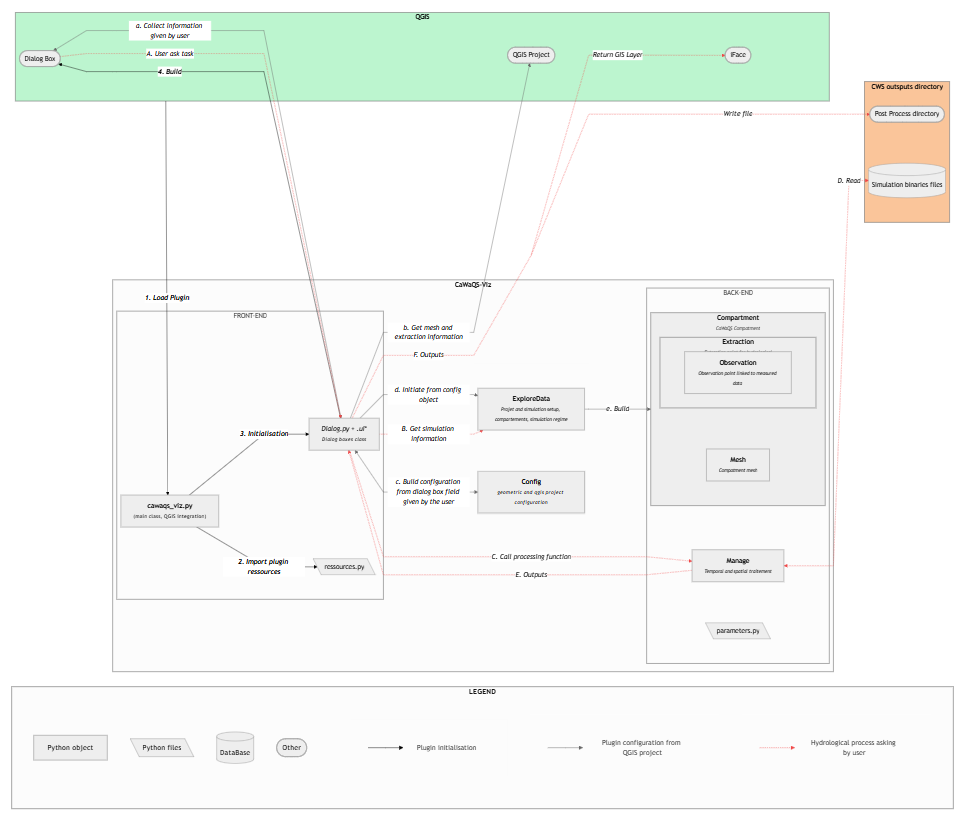
\includegraphics[width=1\linewidth]{5_develloppeur/fig/schema_cwv.png}
    \caption{Schéma fonctionnel de l'application \cwv}
    \label{fig_fonctionnement_cwv}
\end{figure}

\section{Mise à jour de la version} 

La version du plugin est renseignée dans le fichier \script{metadata.txt} contenu dans l'extrait de code \ref{code_metadata}.
\begin{lstlisting}[language=json, caption={Informations obligatoires à renseginer dans le fichier \script{metadata.txt}}, label={code_metadata}]
[general]
name=CaWaQS-Viz
qgisMinimumVersion=3.0
description=Description
version=0.1.16
author=Lise-Marie GIROD (Mines Paris - PSL), Nicolas Flipo (Mines Paris - PSL)
email=lise-marie.girod@minesparis.psl.eu

about=Python QGIS-based vizualization software for CaWaQS3.x

repository=https://gitlab.com/gviz/cawaqsviz
\end{lstlisting}

\section{Documentation du code} 

La documentation du code est publiée sur le lien suivant via gitlab Pages au lien suivant : \href{https://cawaqsviz-gviz-adf347ff6d9d45c174db091497a2dfc0f14305cdb4ed9070.gitlab.io/}{https://cawaqsviz-gviz-adf347ff6d9d45c174db091497a2dfc0f14305cdb4ed9070.gitlab.io/}. L'alimentation de la documentation est assurée par la tenue des docstrings dans les modules de l'application, selon le formatage présenté en exemple. 


\begin{lstlisting}[language=Python, caption={Formatage de la docstring pour intégration automatique dans la documentation du code}, label={code_format_docstrings}]
class Exemple:
    """
    Resume des fonctionnalites de la classe.
    """

    def __init__(self, arg1):
        """
        Methode constructeur.

        :param arg1: descriptif du parametre
        :type arg1: str
        """
        self.arg1 = arg1

    def do_something(self, arg1: list) -> str:
        """
        Descriptif de la fonction.

        :param arg1: descriptif du parametre
        :type arg1: list
        :return: descriptif de ce que la fonction retourne
        :rtype: str
        """
        return ", ".join(map(str, arg1))
\end{lstlisting}
\vspace{1em}
La compilation est opérée par \script{Sphinx}\footnote{dont la documentation est accecible via \href{https://www.sphinx-doc.org/en/master/}{https://www.sphinx-doc.org/en/master/}}. Le répertoire \script{docs/sources} contient les fichiers de configuration (\script{Conf.py}), ainsi que le contenu de la documentation. 
Dans le cas de l'intégration de nouvelles dans le plugin, leur intégration dans l'index (\script{index.rst}) est nécessaire pour que la docstring du code apparaisse dans le page de documentation. Cet index est intègre 3 fichiers  : \script{frontend.rst}, \script{interface.rst}, \script{backend.rst} qui contiennent les classes à documentés. L'intégration d'un nouveau module dans l'application nécessite d'être ajouté dans ces fichiers sous la forme de l'extrait de code \ref{code_format_rst}. Les mises à jour des fichiers sources de la documentation doivent être commité et synchronisé avec les dépôts. 

\begin{lstlisting}[language=Python,caption={Formatage de la docstring pour intégration automatique dans la documentation du code}, label={code_format_rst}]
Module
------

.. automodule:: cawaqsviz.Module
   :members:
   :show-inheritance:
   :undoc-members:
\end{lstlisting}

\vspace{1em}

Finalement à chaque nouveau commit dans les branche \script{Main} ou 
\script{Beta}, la documentation est compilée selon le contenu du répertoire \script{docs/source} du dépôt.

\begin{lstlisting}
image: python:3.9

stages:
  - build
  - deploy

before_script:
  - pip install -U pip
  - pip install -r requirements.txt

build-docs:
  stage: build
  script:
    - sphinx-build -b html docs/source public
  artifacts:
    paths:
      - public

pages:
  stage: deploy
  script:
    - echo "Pages deployed"
  artifacts:
    paths:
      - public
  only:
    - main  
    - beta

\end{lstlisting}

\newpage
\section{Outils de débogage}
\subsection{Le plugin \script{Plugin Reloader}}

Cet utilitaire permet de recharger un plugin après une modification de son code. Ainsi il n'est pas nécessaire de recharger QGIS à chaque modification de code. 

Le plugin est installable depuis le gestionnaire d'extention de \script{QGIS}.

\begin{figure}[H]
    \centering
    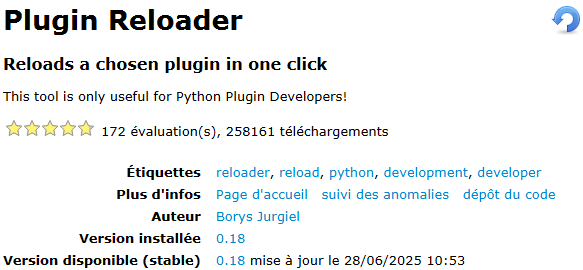
\includegraphics[width=0.75\linewidth]{5_develloppeur/fig/plugin_reloader.png}
    \caption{Fiche descriptive de \script{Plugin Reloader}}
    \label{fig_plugin_reloader}
\end{figure}

\subsection{Le plugin QGIS \script{First Aid}}

Le plugin \script{First Aid} permet d'investiger les erreurs survenant à l'exution du plugin 


\newpage
\subsection{VS-Code}
Le plugin \script{debugvs} permet de connecté une instance de débogage \script{VS-Code} à l’exécution du plugin depuis QGIS. Cette configuration de debugage permet d'utiliser toute les fonctionnalités de VS Code durant le debugague (breakpoint, espion, pile d'appels...).  La mise en place de cette configuration de debugage est réalisée de la manière suivante : 
\begin{enumerate}
    \item installer \script{debugpy} avec la commande \script{!pip install debugpy} depuis l'invité de commande Python de QGIS ;
    \item \sloppy si le répertoire de développement du plugin ne se situe pas dans le répertoire \texttt{C://Users/$USER$/AppData//QGIS/QGIS3/profiles/default/python}, créer un lien symbolique dans ce repertoire pointant vers le répertoire de développement.  
    \item installer le plugin \script{debugvs} en téléchargeant son script depuis le dépôt Gitlab \url{https://github.com/lmotta/debug_vs} et activer le plugin en important le dossier \script{.zip} dans \script{QGIS} (\cffig \ref{fig_debugvs}) ; 
    \begin{figure}[H]
        \centering
        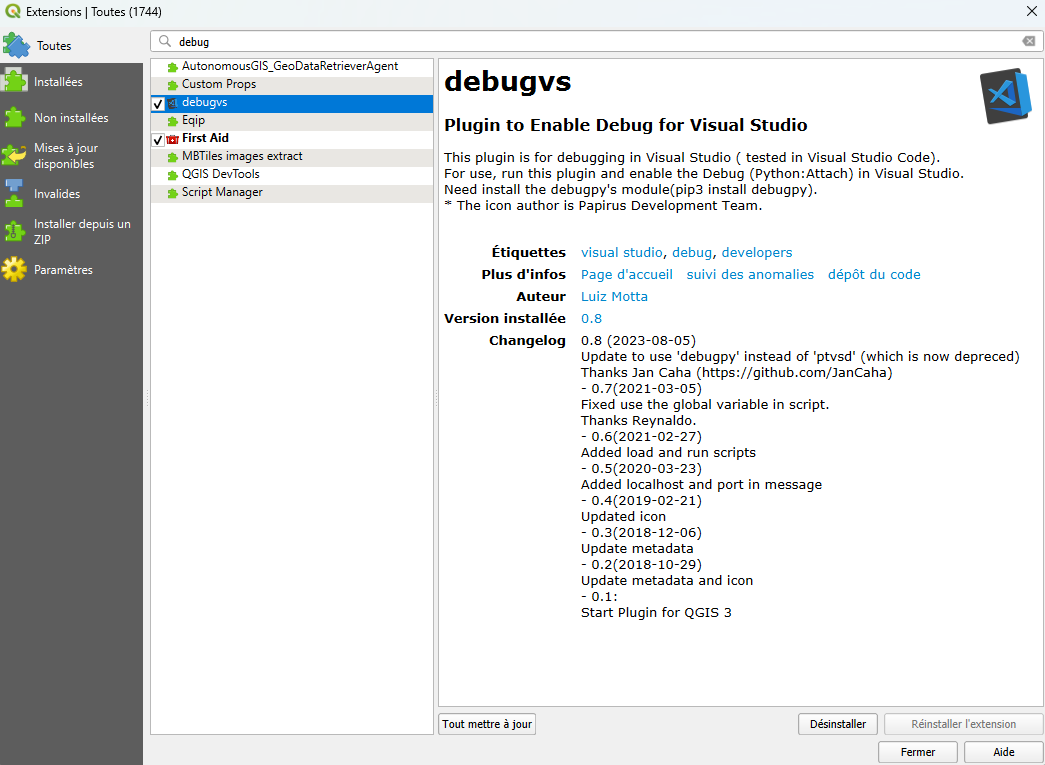
\includegraphics[width=0.6\linewidth]{5_develloppeur/fig/debugvs.png}
        \caption{Pluging \script{debugvs}}
        \label{fig_debugvs}
    \end{figure}
    \item configurer VS Code pour se connecter à QGIS durant une session de debuggage : 
    \begin{enumerate}
        \item dans le répertoire de développement du CaWaQS-Viz, créer un sous-répertoire \script{.vscode} (ajouter ce répertoire au fichier \script{.gitignore}) ; 
        \item créer un fichier \script{settings.json} dans le sous-répertoire \script{.vscode} et copier du contenu du code \ref{code_settings_vscode}.Modifier éventuellement les chemins d'accès au répertoire pour qu'ils correspondent à votre installation de QGIS et de Python et à votre système opératif. Celui-là, c'est pour Windows.
        \begin{lstlisting}[language=JSON, caption={Fichier de configuration du workspace. Ce fichier définit la configuration du workspace Visual Studio Code pour le développement du plugin QGIS. Il permet d’adapter l’environnement Python de VS Code à celui utilisé par QGIS (installé via OSGeo4W).}, label=code_settings_vscode]
        {   
            
            "workbench.colorCustomizations": {
                "titleBar.activeBackground": "#006823",
                "editor.background": "#000000"
            },
            
            "python.linting.pylintEnabled": true,
            "python.jediEnabled": true,
        
            
            "python.pythonPath": "C:/OSGeo4W64/bin/python-qgis.bat",
        
        
            "python.linting.pylintArgs": [
                "--extension-pkg-whitelist=PyQt5,qgis,db_manager",
                "--disable=all",
                "--enable=F,E,unreachable,duplicate-key,unnecessary-semicolon,global-variable-not-assigned,unused-variable,binary-op-exception,bad-format-string,anomalous-backslash-in-string,bad-open-mode"
            ],
        
           
            "terminal.integrated.env.windows": {
                
                "PATH": "C:\\OSGeo4W\\apps\\qgis\\bin;C:\\OSGeo4W\\apps\\Python312;C:\\OSGeo4W\\apps\\Python312\\Scripts;C:\\OSGeo4W\\apps\\Qt5\\bin;C:\\OSGeo4W\\apps\\Python312\\Scripts;C:\\OSGeo4W\\bin;C:\\Windows\\System32;C:\\Windows;C:\\Windows\\system32\\WBem;C:\\OSGeo4W\\apps\\Python312\\lib\\site-packages\\pywin32_system32;C:\\OSGeo4W\\apps\\Python312\\lib\\site-packages\\numpy\\.libs",
                
                "PYTHONHOME": "C:\\OSGeo4W\\apps\\Python312",
                "PYTHONPATH": "C:\\OSGeo4W\\apps\\qgis\\python;%PYTHONPATH%",
                
                "GDAL_DATA": "C:\\OSGeo4W\\share\\gdal",
                "GDAL_DRIVER_PATH": "C:\\OSGeo4W\\bin\\gdalplugins",
                "GDAL_FILENAME_IS_UTF8": "YES",
                
                "GEOTIFF_CSV": "C:\\OSGeo4W\\share\\epsg_csv",
                
                "O4W_QT_BINARIES": "C:/OSGeo4W/apps/Qt5/bin",
                "O4W_QT_DOC": "C:/OSGeo4W/apps/Qt5/doc",
                "O4W_QT_HEADERS": "C:/OSGeo4W/apps/Qt5/include",
                "O4W_QT_LIBRARIES": "C:/OSGeo4W/apps/Qt5/lib",
                "O4W_QT_PLUGINS": "C:/OSGeo4W/apps/Qt5/plugins",
                "O4W_QT_PREFIX": "C:/OSGeo4W/apps/Qt5",
                "O4W_QT_TRANSLATIONS": "C:/OSGeo4W/apps/Qt5/translations",
                "QT_PLUGIN_PATH": "C:\\OSGeo4W\\apps\\qgis\\qtplugins;C:\\OSGeo4W\\apps\\Qt5\\plugins",
                
                "QGIS_PREFIX_PATH": "C:/OSGeo4W/apps/qgis",
                
                "VSI_CACHE": "TRUE",
                "VSI_CACHE_SIZE": "1000000"
            },
            "python.languageServer": "Jedi", 
        }
\end{lstlisting} 
        \item créer un fichier \script{launch.json} dans le sous répertoire \script{.vscode}, copier le contenu du code \ref{code_launch_vscode}, modifier les chemin d'accès \script{localRoot} et \script{remoteRoot} pour correspondre à la configuration de votre espace de travail.
        
        \begin{lstlisting}[language=JSON, caption={Fichier de configuration du debugger VS-Code. Dans cette configuration, la section "connect" indique l’adresse et le port sur lesquels QGIS expose la session de débogage (ici localhost:5678). Le bloc "pathMappings" établit la correspondance entre les chemins locaux du projet ouvert dans VS Code (localRoot) et les chemins utilisés par QGIS pour exécuter le plugin (remoteRoot). Cette correspondance est essentielle pour que les breakpoints placés dans VS Code soient correctement associés aux fichiers réellement exécutés par QGIS.}, label = code_launch_vscode]
{
    "version": "0.2.0",
    "configurations": [
        {
            "name": "Attach QGIS Debug",
            "type": "python",
            "request": "attach",
            "connect": {
                "host": "localhost",
                "port": 5678
            },
            "pathMappings": [
                {
                    "localRoot": "C:\\Program Files\\$QGIS$\\apps\\qgis-ltr\\python\\plugins\\cawaqsviz",
                    "remoteRoot": "C:\\Users\\$USER$\\AppData\\Roaming\\QGIS\\QGIS3\\profiles\\default\\python\\cawaqsviz"
                }
            ],
            "justMyCode": false
        }
    ]
}


\end{lstlisting}
        \end{enumerate}
    \item Établir la connexion QGIS/VS-Code
    \begin{enumerate}
        \item autoriser la connexion du debugueur à QGIS par le plugin \script{debugvs} (\cffig \ref{fig_enable_vscode_qgis}) ;
        \begin{figure}[H] 
            \centering
            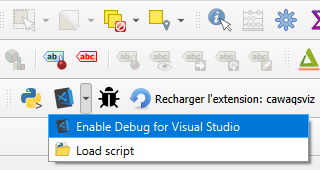
\includegraphics[width=0.40\linewidth]{5_develloppeur/fig/launch_debug_vs.png}
            \caption{Établissement d'une connexion QGIS/VS-Code depuis le plugin \script{debugvs}}
            \label{fig_enable_vscode_qgis}
        \end{figure}
        \item lancer la session de debugage VS-Code (\cffig \ref{fig_debug_VS_CODE}).
        \begin{figure}[H]
            \centering
            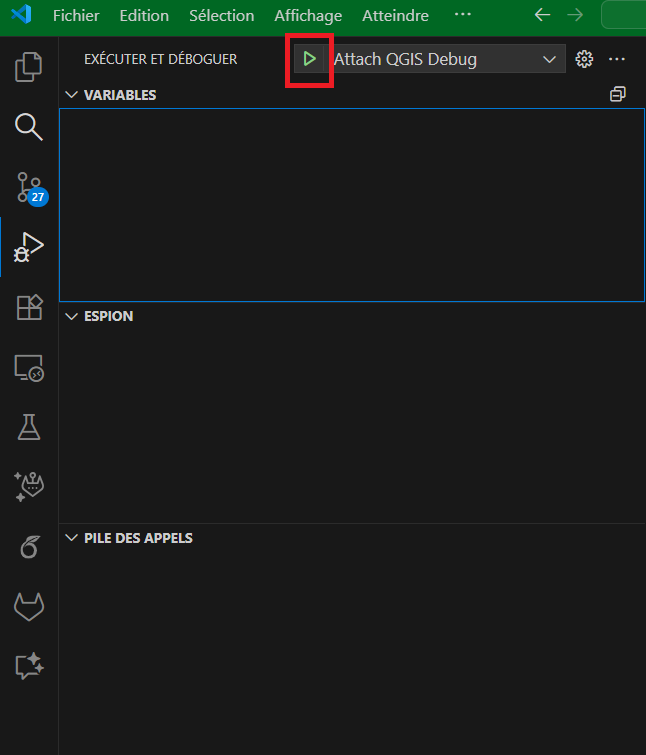
\includegraphics[width=0.5\linewidth]{5_develloppeur/fig/debug_vs_code.png}
            \caption{Lancement d'une session de debuguage depuis VS-Code}
            \label{fig_debug_VS_CODE}
        \end{figure}
    \end{enumerate}
\end{enumerate} 

La connexion entre le debbuger et QGIS est interrompue depuis VS-Code en cliquant sur \script{"Disconnected"} dans la barre d'outil de debuggage (\cffig \ref{fig_barre_outil_debbug}) 

\begin{figure}[H]
    \centering
    
\includegraphics[width=0.35\linewidth]{5_develloppeur/fig/disconnect-debugger.png}
    \caption{Barre d'outil du debugger VS-Code}
    \label{fig_barre_outil_debbug}
\end{figure}






\newpage
\section{Création des boites de dialogue avec \script{Qt Designer}} 
\ref{sec_QtDesigner}
L'application \script{Qt Designer}, livrée à l'installation de QGIS (installation avec OSGEO), est un outil de création de boite de dialogue sous la forme de fichier .ui. Dans l'application \cwv, toutes les boites de dialogues ont leur propre fichier \script{.py} auquel le fichier \script{.ui}, du même nom, est associé à la classe python de la boite de dialogue. 

\begin{lstlisting}[language = Python, label = code_init_from_ui, caption = Initialisation de la boite de dialogue "Compare SIM/OBS" depuis un fichier .ui]
# This loads your .ui file so that PyQt can populate your plugin with the elements from Qt Designer
FORM_CLASS, _ = uic.loadUiType(
    os.path.join(os.path.dirname(__file__), "DialogComparesimobs.ui")
)


class DialogComparesimobs(Dialog, FORM_CLASS):
    def __init__(self, iface:QgisInterface, log_file_path:str, parent=None):
        """Constructor Method

        :param iface: Qgis Interface
        :type iface: QgisInterface
        :param logFilePath: Path of the cawaqs-viz log file, defaults to None
        :type logFilePath: str, optional
        :param parent: Parent class, defaults to None
        :type parent: _type_, optional
        """
        super(DialogComparesimobs, self).__init__(parent)
        self.setupUi(self)
        self.iface = iface
        self.logFilePath = log_file_path
        self.simData = False
\end{lstlisting}

